\documentclass[headings=optiontohead,12pt,letterpaper,oneside,spanish]{book}
\usepackage[spanish, activeacute]{babel}% Utilizamos el paquete para utilizar espa\~nol
\usepackage[utf8]{inputenc}
\usepackage[T1]{fontenc}
\usepackage{lmodern}%Esto evita los problemas derivados al hacer dvipdf con el paquete '[T1]{fontenc}'. The Debian package that includes this fonts should be installed and its name is lmodern.deb

\usepackage{graphicx}% Utilizamos el paquete para gestionar imagenes jpg
\usepackage{amsmath}
\usepackage{amssymb}%Para simbolos matematicos como el \\mathbb{R}
\usepackage{geometry}
\geometry{verbose,letterpaper,tmargin=2.5cm,bmargin=2cm,lmargin=3.5cm,rmargin=2cm}
%\pagestyle{plain}

%Para usar Times New Roman
\usepackage{times}

%%%%%%%%%%%%%%%%%%%%%% Esto es para que la cabecera no quede con todas las letras en mayusculas %%%%%
\usepackage{regexpatch}% http://ctan.org/pkg/regexpatch
\makeatletter
% \*patchcmd{<cmd>}{<search>}{<replace>}{<success>}{<failure>}
\xpatchcmd{\chaptermark}{\MakeUppercase}{}{}{}%
%\xpatchcmd{\sectionmark}{\MakeUppercase}{}{}{}%
%\xpatchcmd*{\tableofcontents}{\MakeUppercase}{}{}{}%
\makeatother
%%%%%%%%%%%%%%%%%%%%%%%%%%%%%%%%%%%%%%%%%%%%%%%%%%%%%%%%%%%%%%%%%%%%%%%%%%%%%%%%%%%%%%%%

%\setcounter{secnumdepth}{3}
%\setcounter{tocdepth}{3}
\usepackage{longtable}
\usepackage{subfigure}
\usepackage{float}
\usepackage{epsfig}
\usepackage{listings}%para escribir codigo C
\usepackage{subfigure}%para figuras una al lado de otras

\makeatletter

\usepackage{algorithm}
\usepackage{algorithmic}

% Para atenuar el corte de palabras
\sloppy 
\hyphenpenalty=10000

%Interlineado en 1.5
\usepackage{setspace}
\spacing{1.5}


%Esto es para que se coloque la palabra 'Algoritmo' en vez de 'Algorithm'
\newfloat{algorithm}{tbp}{loa}
\floatname{algorithm}{Algoritmo}




\begin{document}

%Los 2 comando de a continuacion cambian el nombre 
%"Cuadro" por "Tabla"
\renewcommand{\listtablename}{'Indice de tablas}
\renewcommand{\tablename}{Tabla}

\thispagestyle{empty}

%\begin{flushleft}
\textbf{
\small{
\hspace{-0.2cm}UNIVERSIDAD CATÓLICA DEL MAULE  \\
Facultad de Ciencias de la Ingeniería  \hfill  Profesor Guía\hspace{-0.1cm}\\
Escuela de Ingeniería Civil Informática \hfill  Nombre\_profesor\_Guía\\
}
}
\vspace{5cm}
\begin{center}
		{\bf {\normalsize TÍTULO DE LA TESIS}}\\
\vspace{1cm}
        {\bf {\normalsize NOMBRE(S) ALUMNO(S) TESISTA(S)}}\\
\vspace{1cm}
        {\normalsize Tesis  para optar al}\\
        {\normalsize Título Profesional de Ingeniero Civil Informático}
%\end{flushleft}
\vfill
\textbf{Talca, MES 20XX}
\end{center}

\newpage

\thispagestyle{empty}

\begin{center}
\textbf{
    UNIVERSIDAD CATÓLICA DEL MAULE\\
    FACULTAD DE xCIENCIAS DE LA INGENIERÍA\\
    ESCUELA DE INGENIERÍA CIVIL INFORMÁTICA\\
}
\vspace{1.5cm}

TESIS PARA OPTAR AL\\
TÍTULO PROFESIONAL DE INGENIERO CIVIL INFORMÁTICO\\

\vspace{1.2cm}

``TÍTULO DE LA TESIS''\\
NOMBRE(S) ALUMNO(S) TESISTA(S)\\

\end{center}

\vspace{0.5cm}

%\begin{tabular}{l}
    \textbf{COMISIÓN EXAMINADORA \hfill FIRMA}\hspace*{2cm}\\
%\vspace{0.5cm}

    PROFESOR GUÍA \hfill \\
    NOMBRE\_PROFESOR\_GUÍA \hfill \_\_\_\_\_\_\_\_\_\_\_\_\_\_\_\_\_\_\_\_\_\_\_ \\
%\vspace{0.5cm}

    PROFESOR COMISIÓN \hfill \\
    NOMBRE\_PROFESOR\_COMISIÓN \hfill \_\_\_\_\_\_\_\_\_\_\_\_\_\_\_\_\_\_\_\_\_\_\_ \\
%\vspace{0.5cm}

    PROFESOR COMISIÓN \hfill \\
    NOMBRE\_PROFESOR\_COMISIÓN \hfill \_\_\_\_\_\_\_\_\_\_\_\_\_\_\_\_\_\_\_\_\_\_\_ \\
%\vspace{0.8cm}

    NOTA FINAL EXAMEN DE TÍTULO\hfill \_\_\_\_\_\_\_\_\_\_\_\_\_\_\_\_\_\_\_\_\_\_\_ \\
%\end{tabular}

\vfill

\begin{center}
\textbf{TALCA, MES DE 20XX}
\end{center}




\newpage

%\thispagestyle{empty}

%%%%%    Dedicatoria (Opcional)     %%%%%%%%%%
%\vspace{5cm}
%\begin{flushright}\textbf{\Large A Persona-1 y Persona-2}\end{flushright}



%%%%    Capítulo de Agradecimiento (Opcional)   %%%%%%
%\chapter{Agradecimientos}
%TEXTO
%\begin{flushright}\emph{Autor}, Fecha.\end{flushright}



\chapter*{Sumario}

resumen trabajo.... (máximo 3 páginas)\\

A continuación algunos ejemplos de figuras, referencia, cita, tabla y algoritmo:\\

\begin{figure}
\begin{center}
   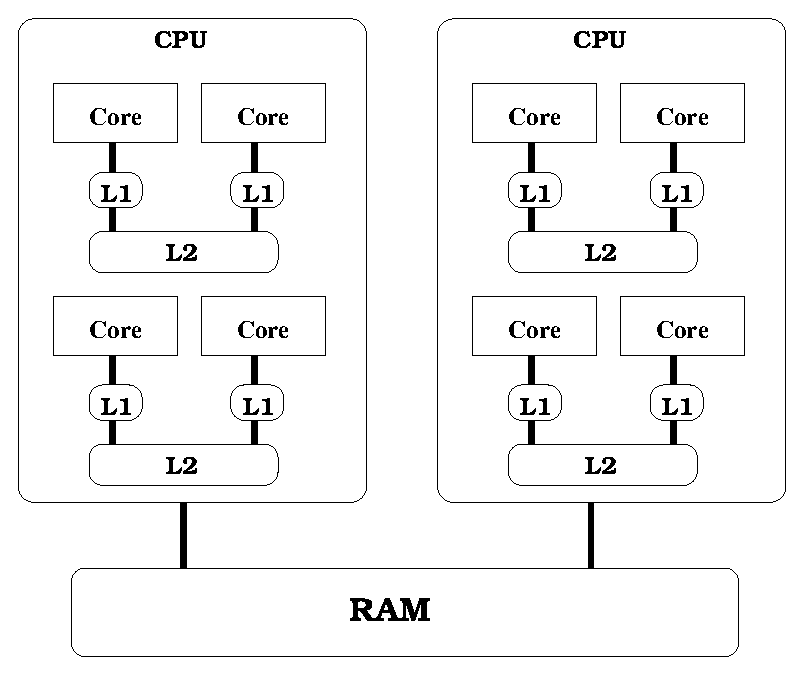
\includegraphics[scale=0.5]{fig/plataforma.eps}
\end{center}
\caption{\label{fig:plataforma}Plataforma multi-core.}
\end{figure}


Una referencia a la Figura \ref{fig:plataforma} y a las subfiguras \ref{cod_gpu_sync-a} y \ref{cod_gpu_sync-b}.
Una cita a libro de Pthreads \cite{libroPthreads}
y OpenMP (\cite{libroOpenMP}).

\begin{figure}
\begin{center}
\subfigure[Caption Subfigura 1]{
	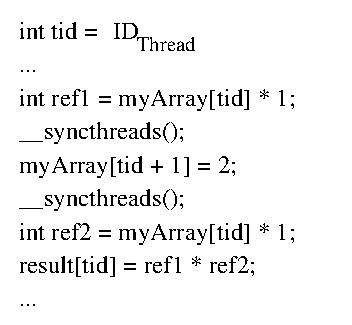
\includegraphics[width=3.5cm,height=4cm]{fig/cod_gpu_sync-a.eps}
    \label{cod_gpu_sync-a}
}~~~~~~~~~~~~
\subfigure[Caption Subfigura 2]{
	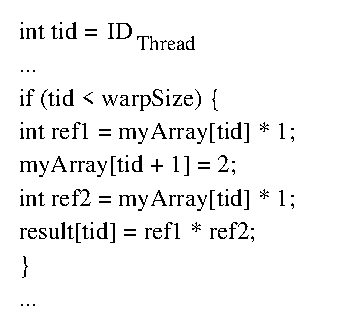
\includegraphics[width=3.5cm]{fig/cod_gpu_sync-b.eps}
    \label{cod_gpu_sync-b}
}
\caption{\label{cod_gpu_sync}Ejemplos para ilustrar la sincronizaci'on
de los threads de un \emph{warp}.}
\end{center}
\end{figure}
%Los caracteres '~' sirven para controlar el espacio entre las figuras. Si están presentes entonces las figuras quedarán una al lado de la otra obligatoriamente.



\begin{algorithm}
busquedarango(Nodo \emph{P}, Consulta \emph{q}, Rango \emph{r})
\footnotesize{
\begin{algorithmic}[1]
\STATE \COMMENT{Sea R el conjunto resultado}
\STATE $R \leftarrow \emptyset$
\STATE $d \leftarrow dist(p_0,q)$
\IF{$d<=r$}
\STATE se reporta $p_0$
\ENDIF
\STATE $range(p_0,q)\leftarrow [d-r,d+r]$
\FORALL {$ x \in P$}
\IF{$range(p_0,q) \cap range(p_0,D_{p_x}) \neq \emptyset$}
\STATE se agrega $x$ a $R$
\IF{$dist(x,q)<=r$}
\STATE se reporta $x$
\ENDIF
\ENDIF
\ENDFOR
\FORALL {$ p_i \in R$}
\STATE busquedarango($D_{p_i}$,q,r)
\ENDFOR

\end{algorithmic}
}
\caption{\emph{\label{cap:ALGgnat:-b=FAsqueda-por-rango}EGNAT}: b'usqueda por
rango $r$ para la consulta $q$.}
\end{algorithm}


   \begin{table}
\begin{center} 
   \caption{\label{tabla_hardware} Caracter'isticas Generales}
   \begin{tabular}{|c|c|}
\hline
   Processor& 2xIntel Quad-Xeon (2.66 GHz)\\
   \hline
   L1 Cache&8x32KB + 8x32KB (inst.+data)\\
   &8-way associative, 64byte per line\\
   \hline
   L2 Unifed Cache&4x4MB (4MB shared per 2 procs)\\
   &16-way associative, 64 byte per line\\
   \hline
   Memory&16GBytes\\
   & (4x4GB) 667MHz DIMM memory\\
   & 1333 MHz system bus\\
   \hline
   Operating System&GNU Debian System Linux\\
   &kernel 2.6.22-SMP for 64 bits\\
   \hline
   \end{tabular}
\end{center}
   \end{table}



\tableofcontents{}

\listoffigures

\listoftables

\listof{algorithm}{\'Indice de Algoritmos}

\mainmatter


%%%  CAPÍTULOS  %%%

\chapter[Introducción]{\label{ch:intro}Introducción}

texto...


\section{Objetivos}

El objetivo general de esta tesis es ....


Los objetivos específicos son los siguientes:

\begin{itemize}
\item objetivo-especifico-1
\item objetivo-especifico-2
\item objetivo-especifico-N
\end{itemize}




\chapter[Estado del Arte]{\label{ch:estado-arte}Estado del Arte}

El paralelimos en computación es una técnica de programación la cual permite que varias intrucciones se puedan ejecutar similtaneamente. Se base en el principio de la división de grandes problemas en varios problemas mas pequeños, que son resueltos de forma concurrente.
\\
\section{Tipos de paralelismo}
Existen diversos tipos de niveles de paralelismo que se describiran a continuación:
\subsection{Nivel de bit}
En la decada de 1970 hasta alrededor de 1986, la aceleración en la arquitectura de computadores lo logro aumentar el tamaño de una palabra, reduciendo asi el numero de instrucciones que un procesador debia realizar, de este modo se logro por ejemplo reducir el proceso de instrucciones en un procesador de 8 bits al sumar dos números de 16 bits.

\subsection{Nivel de instrucción}
Los avances en esta área se realizarón alrededor de 1980 y 1990, donde esto constaba con el reordenamiento y combinación de instrucciones en grupos que luego son ejecutadas en paralelo sin cambiar el resultado del programa. Actualmente los procesadores cuentan con "pipeline" de instrucciones de varias etapas, Cada etapa en el pipeline corresponde a una acción diferente que el procesador realiza en la instrucción correspondiente a la etapa; un procesador con un pipeline de N etapas puede tener hasta n instrucciones diferentes en diferentes etapas de finalización
\subsection{Datos}

El paralelismo de datos es el paralelismo inherente en programas con ciclos, de este modo corresponde a la subdivición de los datos de entrada a un programa, de modo que a cada procesador le corresponda un subconjunto de los datos divididos.\\
Este paradigma es mejor orientado para operaciones con matrices o vectores, debido que se realiza la misma operación sobra cada uno de los elementos.

\subsection{Tareas}

El paralelismo de tareas es la característica de un programa paralelo en la que cálculos completamente diferentes se pueden realizar en cualquier conjunto igual o diferente de datos. Esto contrasta con el paralelismo de datos, donde se realiza el mismo cálculo en distintos o mismos grupos de datos. El paralelismo de tareas por lo general no escala con el tamaño de un problema.
\\

Actualmente la computación paralela ha aumentado su interes debido a las restricciones fisicas, en base a la arquitectura computacional que se han masificados los computadores con procesadores múltinúcleos. Según el hardware que posee el equipo se puede clasificar el nivel de paralelismo que admite, como por ejemplo los computadores multinucleos y multiprocesos permiten realizar varios procesamientos en una misma maquina, mientras que a su vez los clusters, los MPP y los grids emplean varios computadores para trabajar en la misma tarea.
\\
En los ultimos años el uso de coprocesadores ha sido un área de basto interes en temas de investigación en el campo de la computación paralela, con el fin de acelerar procesos secuenciales, los cuales pueden ser acelerados con los procesadores propios del equipo o bien con coprocesadores integrados.

\section{Procesadores y Coprocesadores} 

\subsection{Procesadores}

Un multiprocesador es un conjunto de dos o más procesadores los cuales se encuentran a menudo integrados en un solo circuito. Hoy en día los multiprocesadores mas conocidos son dual-core, quad-core, octa-core con dos, cuatro y ocho núcleos respectivamente. Estos multiprocesadores permiten un paralelismo a nivel de hilos (threads) conocido como TLP (thread-level parallelism), aca no se consideran los microprocesadores en paquetes separados.
\\
Es posible que se realice un procesamiento simultaneo utilizando dos o más procesadores en un pc, o bien realizando la conección de dos o más pc, este ultimo suele ser mas restrintivo debido a las caracteristicas de cada uno de los pcs conectados, que en algunos casos se realiza la superposición entre ellos.

\subsection{Coprocesadores}

Un coprocesador es un microprocesador de un ordenador utilizado como suplemento de las funciones del procesador principal (la CPU). Las operaciones ejecutadas por uno de estos coprocesadores pueden ser operaciones de aritmética, procesamiento gráfico, de señales, procesado de texto o criptografía, etcétera.
\\
Las lineas más famosas de coprocesadores en el ámbito de la investigación son INTEL con su tecnología MIC y NVIDIA GPU con su tecnología CUDA

\subsection{Intel}
Intel a desarrollado una tecnología propía, orientada a computo intensivo en computación paralela conocido como MIC (Many integrated core) asociados a su familia Xeon, similar a la Nvidia Tesla que forman una arquitectura de alto rendimiento. \\
Se puede considerar que cada núcleo del co-procesador Xeon Phi es una unidad de ejecución
multi-hilo completamente funcional. Poseen un rendimiento de hasta 1,2 teraFlops  (operaciones de coma flotante por segundo) por coprocesador para algunas de las aplicaciones más exigentes de hoy día.

\subsection{NVIDIA}
NVIDIA se ha dedicado a la elaboración de GPUs (Unidades de procesamiento gráfico) los cuales son procesadores de varios núcleos que ofrecen un alto rendimiento, tambien dedicados al procesamiento de graficos o bien operaciones de punto flotante. \\
NVIDIA ha desarrollado una tecnología de acuerdo a su hardware conocida como CUDA, que cuenta con una plataforma de computación paralela y un modelo de programación. Esta tecnología permite aumentos considerables en el rendimiento computacional al aprovechar la potencia de la GPU.

\section{KNN (k-nearest neighbors)}

Conocido por sus siglas en ingles como KNN (K-nearest neighbors) k vecinos más cercanos, es un método de clasificación de objetos, siendo la clafisicación de objetos un área muy importante en variados campos de investigación y de aplicaciones, como lo son el reconocimiento de patrones, inteligencia artificial, psicología cognitiva, analísis de videos y medicina.  
\chapter[Marco Teórico]{\label{ch:marco-teorico}Marco Teórico}

bla bla....

\chapter[Desarrollo]{\label{ch:desarrollo}Desarrollo}

\section{\label{sec:des-intro}Introducción}

En este capitulo se describirá el proceso de creación del Software mencionado ya anteriormente en capítulos previos, en los cuales se indica que el software contiene una recopilación de diversos algoritmos K-nn en diferentes plataformas paralelas y además del K-nn secuencial para equipos que no posea las características necesarias para utilizar este software, de este modo se presentara desde la metodología utilizada hasta su desarrollo final con el software en su primera versión terminada. 
Para ello sera necesario describir procesos y etapas que se dividirían en este capitulo.

\section{Desarrollo interfaz}

En esta sección se aborda como se desarrolló la interfaz gráfica, en un principio se estableció \textit{JAVA} como el lenguaje de programación y se utilizo el IDE \textit{netbeans}  \cite{netbeans}, a continuación se explican cada uno de los pasos tomados en consideración al realizar la interfaz gráfica.
\\
En un principio se estableció \textit{JAVA} debido a su capacidad de ser soportado por diversos sistemas operativos, como son Windows, OSx, Linux. Dado que JAVA es un lenguaje interpretado y no compilado, el interpretador (Maquina virtual) de Java es soportado por todos los sistemas antes mencionados, además el uso de \textit{netbeans} permite la fácil creación de una interfaz gráfica, esto debido a poseer \textit{drag and drop} para sus componentes gráficos, en otras palabras solo se necesita arrastrar una componente y situarla en la posición necesaria, esta ventaja dada por \textit{netbeans} es útil, debido al menor tiempo que se ejecuta para crear la interfaz y poder otorgar el tiempo a las funciones correspondientes.\\

Otra característica importante de \textit{JAVA} se debe a que se puede realizar la ejecución de los ejecutables creados luego de la compilación de los algoritmos K-nn y retornar los valores del ejecutable a la interfaz, de esto se logra poder potencial de mejor manera el software. De modo que la interfaz gráfica solo realiza funciones de selección de bases de datos y campos de formularios, en otras palabras la interfaz gráfica solo es una fachada con la finalidad de no realizar la ejecución de los algoritmos desde la terminal.
\\\\
La figura \ref{interfaz_inicial} muestra la interfaz de usuario cuando el software inicia, la cual se compone de la barra superior la cual posee dos menús $"$File$"$ y $"$Menus$"$, una sección de \textit{input} que corresponde a los datos de entrada para el algoritmo K-nn, una sección de \textit{Result} donde en el primer recuadro de la izquierda se muestra la vista previa de las primeras 1000 lineas del archivo de base de datos, en el recuadro central se muestra la vista previa de las primeras 1000 lineas del archivo de consultas, en el cuadro de la derecha muestra los resultados del proceso, muestra si la carga de los datos fue exitosa, el tiempo de ejecución o algún error que pudiese haber ocurrido, como el fallo en la carga de los datos. En la parte inferior del software indica la cantidad de núcleos que posee la maquina donde el software esta instalado.

\begin{figure}[hbtp]
	\centering
	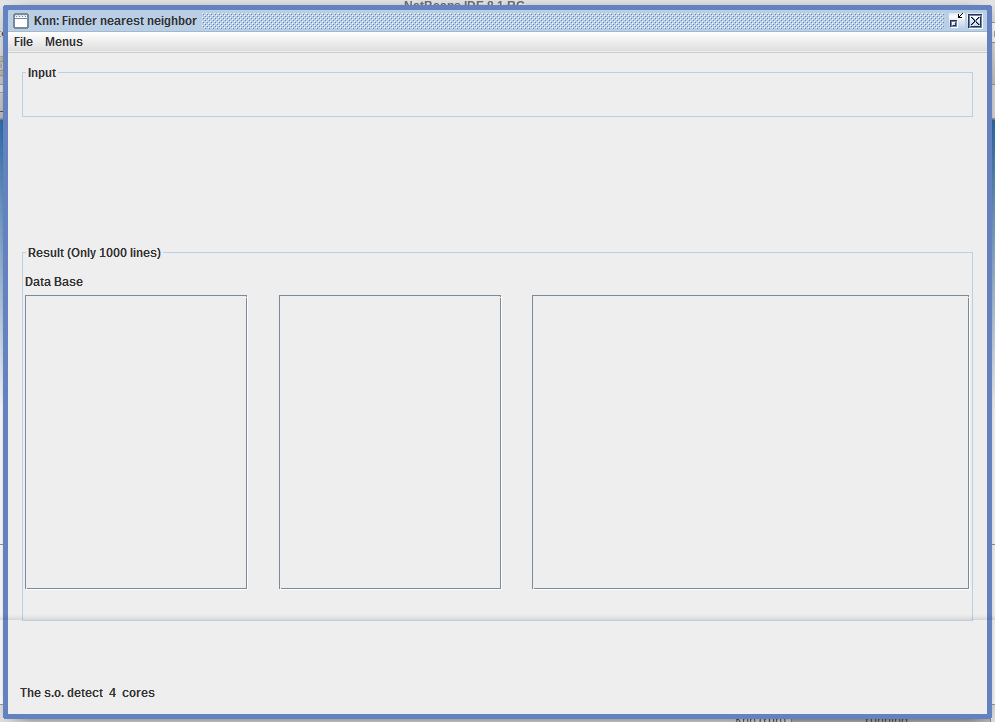
\includegraphics[width=14cm]{fig/interfaz1.png}
	\caption{\label{interfaz_inicial} Interfaz gráfica inicial del software}
\end{figure}      

\subsection*{Menús del software} \label{sec:menu}
El software posee dos menús como se menciono anteriormente, estos corresponden a $"File"$ y $"Menus"$, en el primer menú $File$ posee dos sub-menús $New$ y $Exit$, El primero posee sub-menús que corresponde a los algoritmos que posee el software, estos son:

\begin{itemize}
	\item \textit{Secuencial}
	\item \textit{Multihilos}
	\item \textit{Xeon Phi}
	\item \textit{GPU}
\end{itemize}

Cada uno de estos sub-menús, posee al menos un item que corresponde al algoritmo K-nn programado de acuerdo a la lógica que su nombre indica, esto quiere decir que el sub-menú Multihilos cuenta con a lo menos un item que permite ejecutar el algoritmo K-nn Multihilos, donde este utiliza \textit{OpenMP} para utilizar de mejor manera los recursos de la CPU.\\

Al seleccionar un item del sub-menú \textit{Multihilos} la interfaz gráfica tiene las siguientes características como se aprecia en la figura \ref{interfaz_multihilo}, en la sección $input$ se visualizan los campos de entrada que posee el software, en primer caso es la base de datos, esta se carga mediante el botón examinar, para cargar los datos de consulta se utiliza el botón examinar, $size obj$ es un valor numérico que corresponde a la magnitud del vector ingresado en la base de datos y base de consultas, $K$ es la cantidad de vecinos más cercanos que se desea obtener, $Threads$ por defecto se utiliza la cantidad cantidad de núcleos que posee la maquina donde esta instalado el software, este valor puede ser modificado por la cantidad de hilos que desea el usuario.\\
Además se cuenta con el botón $Start$ para comenzar a ejecutar el las consultas K-nn, se añadió bajo el botón $Start$ un \textit{check box} que permite ejecutar un $Profiler$ que utiliza la librería PapiC \cite{iclit2017} que indica estadísticas sobre el uso de los hilos. En la sección $Result$ no varia en relación al item seleccionado.
 
\begin{figure}[hbtp]
	\centering
	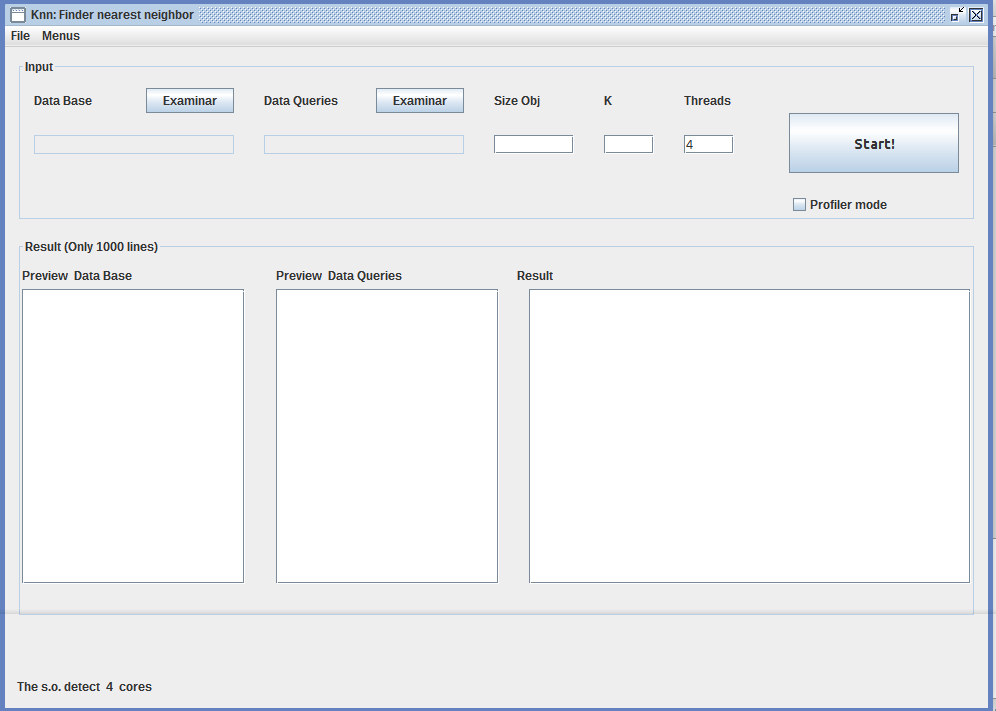
\includegraphics[width=14cm]{fig/interfaz_multicore}
	\caption{\label{interfaz_multihilo} Interfaz gráfica item multihilos del software}
\end{figure}
     
Al seleccionar un item del sub-menú \textit{Secuencial} la interfaz gráfica tiene las siguientes características como se aprecia en la figura \ref{interfaz_secuencial}, en la sección $input$ se visualizan los campos de entrada que posee el software, en primer caso es la base de datos, esta se carga mediante el botón examinar, para cargar los datos de consulta se utiliza el botón examinar, $size obj$ es un valor numérico que corresponde a la magnitud del vector ingresado en la base de datos y base de consultas, $K$ es la cantidad de vecinos más cercanos que se desea obtener.\\

\begin{figure}[hbtp]
	\centering
	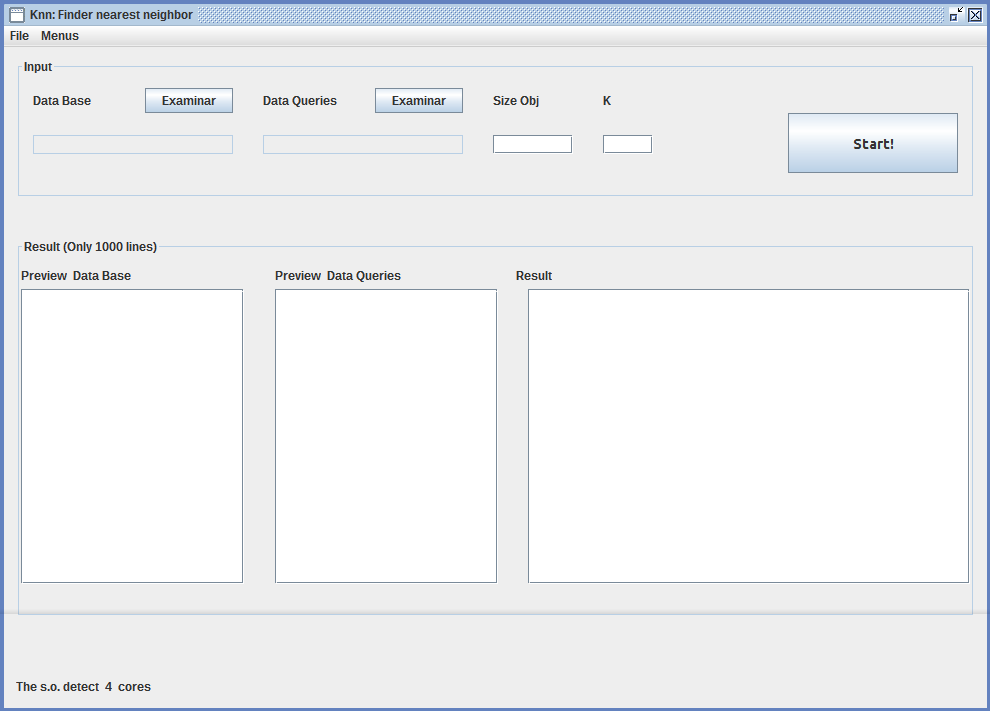
\includegraphics[width=14cm]{fig/interfaz_secuencial}
	\caption{\label{interfaz_secuencial} Interfaz gráfica item secuencial del software}
\end{figure}
 
La selección de los otros item en los sub-menús son similares a los antes mencionados, de modo que solo varia la cantidad de datos de entrada que se ingresan dado las condiciones de programación de cada algoritmo.
\\\\
Además el software cuenta con mensajes dirigidos al usuario, estos son dividen en mensajes de alerta y mensajes de éxito. El primero se aprecia en la figura \ref{mensajes}\subref{fig:error}, este mensaje aparece una vez que se presiona el botón $Start$ y si algún campo esta vacío, indica que campos debe completar para poder ejecutar correctamente el proceso. Si no presenta errores el proceso parte correctamente, si los archivos de bases de datos y consultas son archivos correspondientes, el proceso muestra un mensaje de éxito, como se aprecia en la figura \ref{mensajes}\subref{fig:exito}, al presionar el botón aceptar se muestra la ventana de los resultados de la consulta K-nn, este paso corresponde a la sección \ref{sec:resultados} \textit{Métodos de exportación de resultados}.  

\begin{figure}
\begin{center}
\caption{\label{mensajes} Mensajes al usuario }
\subfigure[Mensaje 1 - Error]{
	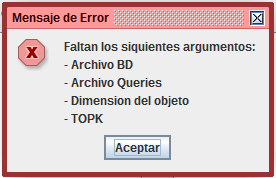
\includegraphics[width=5cm]{fig/error}
    \label{fig:error}
}~~~~~~~~~~~~
\subfigure[Mensaje 2 - Éxito]{
	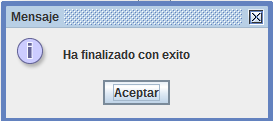
\includegraphics[width=5cm]{fig/exito_knn}
    \label{fig:exito}
}
\end{center}
\end{figure}

\section{Integración de algoritmo K-nn Secuencial} \label{met:secuencial}

Si bien este algoritmo, no estaba considera en un comienzo este se añadió para la posibilidad de poder ejecutar el software en equipos que no cuenten con procesadores con multi-núcleos y necesiten realizar consultas K-nn. Este algoritmo se realizado con la estructura heap \ref{sec:heap}.\\
Para implementar el algoritmo K-nn secuencial, se definió la estructura heap, la cual se aprecia en el segmento de código en el algoritmo \ref{lst:heap}, este almacena en $doble$ $dist$, la distancia del elemento consultado esta es de tipo $double$ debido a que las distancias son reales y puede ser el caso que se necesite almacenar un valor muy grande, a su ves $int ind$ indica la posición del vector dentro de la base de consultas. Cabe recalcar que solo se almacenan K resultados en esta estructura, además de solo almacenar los valores cuya distancia $dist$ sean las k menores.
\\ 
\begin{algorithm}
\begin{lstlisting}[language=C] 
struct _Elem {
    double dist;
    int ind;
};
typedef struct _Elem Elem;
\end{lstlisting}
\caption{\emph{\label{lst:heap}} Estructura para realizar los $Heap$.}
\end{algorithm}

Con el lenguaje de programación C, es posible utilizar la cantidad de memoria justa gracias a la instrucción $malloc$ que permite asignar la cantidad de memoria que corresponde al tamaño de la base de datos y la base de consulta, tal como se aprecia en el algoritmo \ref{lst:malloc}. Donde $consultas$ se crea una matriz de $N\_queries x DIM$ donde $N\_queries$ es el número tuplas de vectores contenidas en la base de consulta y $DIM$ es el tamaño del vector. De manera análoga se establece la matriz $DB$ de $N\_DB x DIM$ donde $N\_DB$ es el número tuplas de vectores contenidas en la base de datos y $DIM$ es el tamaño del vector. A su vez $answer$ corresponde a la asignación de memoria para las $N\_queries$ con $K$ vecinos más cercanos donde se almacenan todas las respuestas a las consultas para ser finalmente mostrados. $Heap$ es la estructura a utilizar con cada consulta, esta corresponde a un heap del tipo heap max, donde el nodo padre es el mayor valor de la estructura.
\\
El desarrollo central del algoritmo para obtener los k vecinos más cercanos esta dado por el algoritmo \ref{lst:knn}, este algoritmo indica las siguientes acciones, se establece un contador $n\_elem$ $=0$ que obtiene el número de elementos que han ingresado al heap, este se utiliza como comparador debido a que se deben ingresar k elementos al heap, mientras $n\_elem$ sea menor que el número $k$ se ingresaran los datos al heap en caso contrario se compara si la distancia del elemento actual es menor a la raíz del heap de manera que si el elemento es menor se extrae la raíz y se añade el elemento actual y se reordena el heap. Este proceso itera exhaustivamente hasta que no queden elementos en la base de datos, cuando el heap esta finalizado se almacenan sus resultados en la matriz $answer$ y se debe continuar con la siguiente consulta hasta que se realicen todas las consultas del base de consultas.

\begin{algorithm}
\begin{lstlisting}[language=C]
    Consultas = (double **) malloc(sizeof (double *)*N_QUERIES);
    for (i = 0; i < N_QUERIES; i++)
        Consultas[i] = (double *) malloc(sizeof (double)*DIM);

    DB = (double **) malloc(sizeof (double *)*N_DB);
    for (i = 0; i < N_DB; i++)
        DB[i] = (double *) malloc(sizeof (double)*DIM);

    answer = (Elem *)malloc(sizeof(Elem)*N_QUERIES*TOPK);
    
    heap = (Elem *) malloc(sizeof (Elem) * TOPK);
\end{lstlisting}
\caption{\emph{\label{lst:malloc}} Utilización de $malloc$.}
\end{algorithm}


\begin{algorithm}
\begin{lstlisting}[language=C]
for (i = 0; i < N_QUERIES; i++) {
	n_elem = 0;
	for (j = 0; j < N_DB; j++) {    
		d = distancia(Consultas[i], DB[j]);
		if(n_elem<TOPK){
			e_temp.dist = d;
			e_temp.ind = j;
			inserta2(heap, &e_temp, &n_elem);
		}
		else{
			if (d < topH(heap, &n_elem)) {
				e_temp.dist = d;
             	e_temp.ind = j;
				popush2(heap, &n_elem, &e_temp);
		}}
	}
        for (int k = 0; k < TOPK; ++k){
        	extrae2(heap, &n_elem, &e_temp);
        	answer[i*TOPK+k].ind = e_temp.ind;
        	answer[i*TOPK+k].dist = e_temp.dist;
        }
}
\end{lstlisting}
\caption{\emph{\label{lst:knn}} Proceso iterativo de una consulta K-nn.}
\end{algorithm}

\subsection{Funciones claves del algoritmo secuencial}  \label{met:claves}

$Distancia:$ Algoritmo \ref{lst:distancia} es la función de cálculo de la distancia entre vectores, tanto del vector de la base de datos y el vector de la base de consultas, este cálculo se realiza con la formula \eqref{ecu:distancia}.\\
Dados $A$ = $(X_1,Y_1)$ y $B$ = $(X_2,Y_2)$

\begin{equation}\label{ecu:distancia}
 distancia = \sqrt{(X_2-X_1)^{2}+(Y_2-Y_1)^{2}}
\end{equation}

Esta ecuación puede ser llevada a vectores de tamaño $n$.

\begin{algorithm}
\begin{lstlisting}[language=C]
double distancia(double *p1, double *p2) {
    int i = 0;
    double suma = 0;

    for (i = 0; i < DIM; i++)
        suma += ((p1[i] - p2[i])*(p1[i] - p2[i]));
    return sqrt(suma);
}  
\end{lstlisting}
\caption{\emph{\label{lst:distancia}} Cálculo de distancias entre vectores.}
\end{algorithm}


Sumado a esta función existen las funciones para manipular un heap, estas corresponden a obtener el valor nodo padre (Algoritmo \ref{lst:top}), realizar una inserción de un elemento, extraer un elemento y una añadida para facilitar el procedimiento del algoritmo como es el caso de una extracción e inserción que se utiliza cuando se debe cambiar un nodo dentro del heap y realizar el reordenamiento del heap.
\\
El algoritmo \ref{lst:top} retorna el valor de la raíz (nodo padre) del heap si no esta vacío, en caso contrario retorna el valor maximo de un $double$.
   
\begin{algorithm}
\begin{lstlisting}[language=C]
double topH(Elem *heap, int *n_elem) {
    if (*n_elem == 0)
        return DBL_MAX;
    return heap[0].dist;
}
\end{lstlisting}
\caption{\emph{\label{lst:top}} Valor de la raíz del heap.}
\end{algorithm}

El algoritmo \ref{lst:inserta2} realiza la inserción de un elemento, guardando la distancia y la posición del elemento, el contador $n\_elem$ incrementa en 1 luego de la inserción, y se realiza el ordenamiento del heap. Esta función es la que se utiliza en el algoritmo \ref{lst:heap} hasta llenar el heap.

\begin{algorithm}
\begin{lstlisting}[language=C]
void inserta2(Elem *heap, Elem *elem, int *n_elem) {
    int i;
    Elem temp;

    heap[*n_elem].dist = elem->dist;
    heap[*n_elem].ind = elem->ind;
    (*n_elem)++;
    for (i = *n_elem; i > 1 && heap[i - 1].dist > heap[(i / 2) - 1].dist; i = i / 2) {
        temp = heap[i - 1];
        heap[i - 1] = heap[(i / 2) - 1];
        heap[(i / 2) - 1] = temp;
    }
}
\end{lstlisting}
\caption{\emph{\label{lst:inserta2}} Realiza la inserción de un elemento al heap.}
\end{algorithm}

El algoritmo \ref{lst:extrae2} realiza la extracción de un elemento, guardando la distancia y la posición del elemento, el contador $n\_elem$ decrementando en 1 luego de la extracción, y se realiza el ordenamiento del heap. Esta función es la que se utiliza para completar la matriz $answer$.

\begin{algorithm}
\begin{lstlisting}[language=C]
void extrae2(Elem *heap, int *n_elem, Elem *elem_extraido) {
    int i, k;
    Elem temp;

    (*elem_extraido).dist = heap[0].dist;
    (*elem_extraido).ind = heap[0].ind;

    heap[0] = heap[(*n_elem) - 1]; // Movemos el ultimo a la raiz y achicamos el heap
    (*n_elem)--;
    i = 1;
    while (2 * i <= *n_elem) // mientras tenga algun hijo
    {
        k = 2 * i; //el hijo izquierdo
        if (k + 1 <= *n_elem && heap[(k + 1) - 1].dist > heap[k - 1].dist)
            k = k + 1; //el hijo derecho es el mayor
        if (heap[i - 1].dist > heap[k - 1].dist)
            break; //es mayor que ambos hijos

        temp = heap[i - 1];
        heap[i - 1] = heap[k - 1];
        heap[k - 1] = temp;
        i = k; //lo intercambiamos con el mayor hijo
    }
    return;
}
\end{lstlisting}
\caption{\emph{\label{lst:extrae2}} Realiza la extracción de un elemento al heap.}
\end{algorithm}

El algoritmo \ref{lst:popush2} realiza la extracción del elemento raíz y la posterior inserción del elemento cuya distancia era menor que la distancia del elemento raíz, esta función guarda la distancia y la posición del elemento, con esto luego se realiza el ordenamiento del heap. Esta función es la que se utiliza en el algoritmo \ref{lst:heap}  cuando el heap esta lleno y se obtiene un elemento cuya distancia es menor a la distancia de la raíz.


\begin{algorithm}
\begin{lstlisting}[language=C]

void popush2(Elem *heap, int *n_elem, Elem *elem) {
    int i, k;
    Elem temp;

    heap[0].dist = elem->dist;
    heap[0].ind = elem->ind;

    i = 1;
    while (2 * i <= *n_elem) // mientras tenga algun hijo
    {
        k = 2 * i; //el hijo izquierdo
        if (k + 1 <= *n_elem && heap[(k + 1) - 1].dist > heap[k - 1].dist)
            k = k + 1; //el hijo derecho es el mayor
        if (heap[i - 1].dist > heap[k - 1].dist)
            break; //es mayor que ambos hijos

        temp = heap[i - 1];
        heap[i - 1] = heap[k - 1];
        heap[k - 1] = temp;
        i = k; //lo intercambiamos con el mayor hijo
    }
    return;
}

\end{lstlisting}
\caption{\emph{\label{lst:popush2}} Realiza la extracción y la inserción de un elemento al heap.}
\end{algorithm}

Para realizar la integración de este algoritmo en la interfaz gráfica se realizó mediante una rutina de $Java$ con $java.lang.Runtime.exec()$. La implementación de esta rutina permite ejecutar otro programa o ejecutable y obtener los resultados para ser visualizados a través de la interfaz gráfica creada en $Java$. El algoritmo \ref{lst:javarun} muestra un ejemplo simple de ejecutar un programa o ejecutable desde $Java$.

\begin{algorithm}
\begin{lstlisting}[language=Java]

import java.io.*;
 
public class llamarruntime
{
   public static void main(String[] args)
   {
      try{
         Process theProcess =
                 Runtime.getRuntime().exec(Ejecutable);
      }
      catch(IOException e){
         System.err.println("Error en el metodo exec()");
         e.printStackTrace();
      }
   } 
}
\end{lstlisting}
\caption{\emph{\label{lst:javarun}} Ejecutar un programa o ejecutable desde $Java$.}
\end{algorithm}


\section{Integración de algoritmo K-nn Paralelo Multi-hilos}


Este algoritmo a posee ciertas semejanzas y diferencias con respecto a la versión secuencial, este utiliza $malloc$ como se indica en el algoritmo \ref{lst:malloc}, estableciendo los mismos atributos y designando la memoria de la misma manera que la versión secuencial, léase \ref{met:secuencial}.
\\

A través de la librería \textit{OpenMP} establece variables de tipo compartida \textit{Shared} y variables del tipo privadas \textit{Private}, donde con una variable del tipo compartida se puede obtener su valor o realizar alguna modificación sin restricciones desde cualquier hilo, a su vez una variable del tipo privada solo puede ser accesible por un hilo y se crea una copia de la variable para tantos hilos creados existan. De esta manera se han establecido variables solo variables del tipo \textit{Shared} para este algoritmo.

El desarrollo central del algoritmo para obtener los k vecinos más cercanos esta dado por el algoritmo \ref{lst:knn2}, este algoritmo indica las siguientes acciones, se establece un contador $n\_elem$ $=0$ que obtiene el número de elementos que han ingresado al heap, este se utiliza como comparador debido a que se deben ingresar k elementos al heap, mientras $n\_elem$ sea menor que el número $k$ se ingresaran los datos al heap en caso contrario se compara si la distancia del elemento actual es menor a la raíz del heap de manera que si el elemento es menor se extrae la raíz y se añade el elemento actual y se reordena el heap. Este proceso itera paralelamente hasta que no queden elementos en la base de datos, cuando el heap esta finalizado se almacenan sus resultados en la matriz $answer$ y se debe continuar con la siguiente consulta hasta que se realicen todas las consultas del base de consultas.

\begin{algorithm}
\begin{lstlisting}[language=C]
#pragma omp master
for (i = tid; i < N_QUERIES; i += procs) {           
	n_elem = 0;
    for (j = 0; j < N_DB; j++) {           
    	d = distancia(Consultas[i], DB[j]);               
        if(n_elem<TOPK){
        	e_temp.dist = d;
        	e_temp.ind = j;
        	inserta2(heap, &e_temp, &n_elem);
        }
        else{
        	if (d < topH(heap, &n_elem)) {
            	e_temp.dist = d;
            	e_temp.ind = j;
            }}
        }
        for (j = 0; j < TOPK ; j++) {
        	extrae2(heap, &n_elem, &e_temp);
        	answer[i*TOPK+j].ind = e_temp.ind;
        	answer[i*TOPK+j].dist = e_temp.dist;
       	}
}

#pragma omp barrier
\end{lstlisting}
\caption{\emph{\label{lst:knn2}} Proceso iterativo de una consulta K-nn multi-core.}
\end{algorithm}

A diferencia del método secuencial, el método multi-paralelo utiliza la librería OpenMP, por tanto como se muestra en el algoritmo \ref{lst:knn2} \textit{\#pragma omp master} indica el trabajo en la zona paralela, de manera que el ciclo $for$ realiza un paso cíclico con una cantidad determinada de hilos dada por $procs$, donde $tid$ es el identificador de cada hilo, esto quiere que decir que si utilizo 2 hilos el hilo 0 con $tid=0$ realiza la consulta 0 y el hilo 1 con $tid=1$ realiza la consulta 1 simultáneamente finalizado el trabajo de al menos uno de estos, el hilo con su actividad finalizada toma el valor correspondiente, en caso del hilo 0 con $tid=0$ le corresponde tomar la consulta 2 y al hilo 1 con $tid=1$ le corresponde el hilo 3. Este proceso se realiza hasta llegar al final de la base de consultas $N\_queries$.\\

\subsection{Funciones claves del algoritmo multi-hilos}  

Estas funciones son las mismas que el método secuencial, donde se consideran $topH$ para saber el valor del del nodo raíz, $inserta2$ para insertar un nodo en un heap con el número de elementos menor al de k elementos, $extrae2$ extrae el nodo raíz del heap, $popush2$ realiza la extracción del nodo raíz e inserción de un nuevo nodo de menor valor que la raíz extraída, léase \ref{met:claves}
\\
Para realizar la integración de este algoritmo en la interfaz gráfica se realizó mediante una rutina de $Java$ con $java.lang.Runtime.exec()$. La implementación de esta rutina permite ejecutar otro programa o ejecutable y obtener los resultados para ser visualizados a través de la interfaz gráfica creada en $Java$. El algoritmo \ref{lst:javarun} muestra un ejemplo simple de ejecutar un programa o ejecutable desde $Java$.
 

\section{Integración de algoritmo K-nn Paralelo Xeon Phi}

A diferencia de los métodos anteriores acá se utiliza un coprocesador, de modo que se debe realizar la comunicación entre la CPU y el Coprocesador (\textit{Intel Xeon Phi}). A continuación se describe en detalle las funciones de este método.\\

Con el lenguaje de programación C, es posible utilizar la cantidad de memoria justa gracias a la instrucción $malloc$ que permite asignar la cantidad de memoria que corresponde al tamaño de la base de datos y la base de consulta, tal como se aprecia en el algoritmo \ref{lst:mallocxeon}. Donde $queries$ se crea una matriz de $num\_queries x dimaux$ donde $num\_queries$ es el número tuplas de vectores contenidas en la base de consulta y $dimaux$ es el tamaño del vector. De manera análoga se establece la matriz $db$ de $num\_db x dimaux$ donde $num\_db$ es el número tuplas de vectores contenidas en la base de datos y $dimaux$ es el tamaño del vector. A su vez $answer$ corresponde a la asignación de memoria para las $num\_queries$ con $K$ vecinos más cercanos donde se almacenan todas las respuestas a las consultas para ser finalmente mostrados. $Heap$ es la estructura a utilizar con cada consulta, esta corresponde a un heap del tipo heap max, donde el nodo padre es el mayor valor de la estructura. La Xeon phi permite solo permite realizar el trabajo con vectores de modo que las matrices deben ser trabajadas como vectores y además los vectores deben ser múltiplos de 16, de modo que para solucionar este problema y poder trabajar con la medida de cualquier vector de entrada se parametriza a su vector multiplo de 16 superior, en otras palabras si ingresa un vector de tamaño 8 se parametriza a 16, si ingresa un vector 17 se parametriza a 32 y los valores restantes son establecidos como 0, para no interferir en el cálculo de la distancia.  
\\
El desarrollo central del algoritmo para obtener los k vecinos más cercanos esta dado por el algoritmo \ref{lst:knnxeon}, este algoritmo indica las siguientes acciones, las operaciones de este algoritmo están dentro de la región paralela de la \textit{Xeon phi} (\textit{\#pragma}) de manera que se deben enviar desde la CPU a la \textit{Xeon phi} todas las variables o constantes a utilizar, donde se deben cumplir ciertas restricciones como vectorizar la matriz (explicado anteriormente), además se especifican claramente cuales son datos exclusivamente de entrada \textit{In} y exclusivamente datos de salida \textit{Out} o datos que pueden ser de entrada y salida \textit{(Inout)}. La \textit{Xeon phi} a través de la librería \textit{OpenMP} utiliza además variables de tipo compartida \textit{Shared} y variables del tipo privadas \textit{Private}, donde una variable del tipo compartida puede obtener su valor o realizar alguna modificación sin restricciones, a su vez una variable del tipo privada solo puede ser accesible por un hilo y se crea una copia de la variable para tantos hilos creados existan. A diferencia del método anterior que solo utilizaba variables tipo \textit{Shared}, en este método las variables del tipo \textit{Private} se han establecido las siguientes variables \textit{i, j, thread\_num} de modo que cada hilo puede realizar independientemente sus iteraciones en los ciclos sin ser interrumpido por otro, esto debido a que se utilizan vectores y se debe emular la lectura de la matriz a través de los vectores. Dentro de la región paralela \textit{\#pragma omp parallel} se crea un heap de tamaño \textit{K}. luego se establece un contador $n\_elem$ $=0$ que obtiene el número de elementos que han ingresado al heap, este se utiliza como comparador debido a que se deben ingresar k elementos al heap, mientras $n\_elem$ sea menor que el número $k$ se ingresaran los datos al heap en caso contrario se compara si la distancia del elemento actual es menor a la raíz del heap de manera que si el elemento es menor se extrae la raíz y se añade el elemento actual y se reordena el heap. Este proceso itera paralelamente hasta que no queden elementos en la base de datos, cuando el heap esta finalizado se almacenan sus resultados en la matriz $answer$. Este proceso dentro de la región paralela \textit{\#pragma omp parallel} realiza cada uno de los pasos mencionados por cada hilo utilizado en el proceso\\



 \begin{algorithm}
\begin{lstlisting}[language=C]
   db= (double **)malloc(sizeof(double *)*num_db);
   for (i=0; i<num_db; i++)
      db[i] = (double *)malloc(sizeof(double)*dimaux);
   queries = (double **)malloc(sizeof(double *)*num_queries);
   for (i=0; i<num_queries; i++)
      queries[i] = (double *)malloc(sizeof(double)*dimaux);
   answer = (Elem *)malloc(sizeof(Elem)*num_queries*k);

   //Se transfieren datos de una matriz a un vector
   db_vector = (double *)_mm_malloc(sizeof(double)*dimaux*num_db, 64);
   for (i=0; i < dimaux*num_db; i++)
       db_vector[i] = 0.0;
   if (sizeof(double)*dimaux*num_queries < 64)
   {
        queries_vector = (double *)_mm_malloc(sizeof(double)*16, 64);
        for (i=0; i < 16; i++)
            queries_vector[i] = 0.0;
   }
   else
   {
        queries_vector = (double *)_mm_malloc(sizeof(double)*dimaux*num_queries, 64);
        for (i=0; i < dimaux*num_queries; i++)
            queries_vector[i] = 0.0;
   }
\end{lstlisting}
\caption{\emph{\label{lst:mallocxeon}}  Utilización de $malloc$.}
\end{algorithm}

 \begin{algorithm}
\begin{lstlisting}[language=C]
   #pragma offload target(mic:0) in(dim) in(db_vector:length(num_db*dimaux)) in(queries_vector:length(num_queries*dimaux)) out(answer:length(k*num_queries))
   {
      #pragma omp parallel private(i, j, thread_num) shared(db_vector, num_db, queries_vector, num_queries, dimaux, k, answer, num_threads)
      {
         
         Elem *heap;
         heap = (Elem *)malloc(sizeof(Elem)*k);
         #pragma omp master
         {
            num_threads = omp_get_num_threads();
            printf("run with %d threads\n", num_threads);
         }
         #pragma omp barrier
         thread_num = omp_get_thread_num();
         int n_elem;
         Elem e_temp;
         double d;

         
         for(i=thread_num*dimaux; i<num_queries*dimaux; i+=num_threads*dimaux){
            n_elem = 0;
            for(j=0; j<k; j++){
               e_temp.dist = distancia(&(queries_vector[i]), &(db_vector[j*dimaux]), dimaux);
               e_temp.ind = j;
               inserta2(heap, &e_temp, &n_elem);
            }

            for(j=k; j<num_db; j++){
               d = distancia(&(queries_vector[i]), &(db_vector[j*dimaux]), dimaux);
               if(d < topH(heap, &n_elem))
                  {
                     e_temp.dist = d;
                     e_temp.ind = j;
                     popush2(heap, &n_elem, &e_temp);
                  }
            }

            for(j=0; j<k; j++){
               extrae2(heap, &n_elem, &e_temp);
               printf("%d ind = %d :: dist = %f posicion:: %d \n", j, e_temp.ind, e_temp.dist,(i/dimaux)*k+j);
               answer[(i/dimaux)*k+j].ind = e_temp.ind;
               answer[(i/dimaux)*k+j].dist = e_temp.dist;
            }


         }
         free(heap);
      }
   }   
\end{lstlisting}
\caption{\emph{\label{lst:knnxeon}} Proceso iterativo de una consulta K-nn Xeon phi.}
\end{algorithm}


\subsection{Funciones claves del algoritmo Xeon phi}

A diferencia de los métodos anteriores donde solo se utiliza una \textit{CPU}, aca se emplea tanto la \textit{CPU} como un \textit{Coprocesador} el cual solo realiza tareas especificas (léase \ref{cap:coprocesadores}). A continuación se detallan las principales funciones que se implementaron en \textit{Xeon phi}.\\ 

$Distancia:$ Algoritmo \ref{lst:distanciaxeon} es la función de cálculo de la distancia entre vectores, tanto del vector de la base de datos y el vector de la base de consultas, este cálculo se realiza con la formula \eqref{ecu:distancia}. Esta función se realiza en la \textit{Xeon phi} para indicar que se realizara en el coprocesador se utiliza la sintaxis \textit{\textbf{\_\_atribute\_\_((target(mic)))}}. Las sintaxis \textit{\textbf{\_\_assume\_aligned(), \#pragma vector aligned, \#pragma ivdep, \#pragma simd }} alinea los vectores y permite que el cálculo de la distancia se realice correctamente.
  
\begin{algorithm}
\begin{lstlisting}[language=C]
__attribute__((target(mic))) double distancia(double *p1, double *p2, int DIM){
    int i=0;
    double suma=0.0;
   __assume_aligned(p1, 64);
   __assume_aligned(p2, 64);   
    #pragma vector aligned
    #pragma ivdep
    #pragma simd
    for (i=0; i < DIM; i++){
        suma += (p1[i]-p2[i])*(p1[i]-p2[i]);
    }
    return sqrt(suma);
}
\end{lstlisting}
\caption{\emph{\label{lst:distanciaxeon}} Función distancia \textit{Xeon phi}.}
\end{algorithm}

Debido a que la \textit{Xeon phi} no permite la utilización de matrices se implementa la función \textit{matrixToVector} (Algoritmo \ref{lst:distanciaxeon}) para traspasar la matriz a vector, esta función corresponde a la CPU no a la \textit{Xeon phi} de manera que no utiliza sintaxis especiales.

\begin{algorithm}
\begin{lstlisting}[language=C]
void matrixToVector(double **matrix, int num_cols, int num_rows, double *vector){
    int i,j;
    for(i=0; i<num_rows; i++)
        for(j=0; j<num_cols; j++)
            vector[(i*num_cols)+j] = matrix[i][j];
}
\end{lstlisting}
\caption{\emph{\label{lst:distanciaxeon}} Pasa una matriz a vector.}
\end{algorithm}

De manera similar a los métodos anteriores (Secuencial y Multi-núcleo) se emplean las mismas funciones, pero estas no se ejecutan en la CPU, estas se ejecutan en el \textit{Coprocesador} para esto se añade al principio de cada función la sintaxis \textit{\textbf{\_\_atribute\_\_((target(mic)))}} por ejemplo el algoritmo \ref{lst:topxeon} que devuelve la raíz del heap, solo varia en la sintaxis indicada anteriormente. A su vez tanto $inserta2$, $extrae2$, $popush2$, se deben ejecutar en la \textit{Xeon phi} de modo que se debe añadir al principio de cada función la sintaxis \textit{\textbf{\_\_atribute\_\_((target(mic)))}}.\\\\

\begin{algorithm}
\begin{lstlisting}[language=C]
__attribute__((target(mic))) double topH(Elem *heap, int *n_elem)
{
    if ((*n_elem) == 0)
        return MAXDOUBLE;
    return heap[0].dist;
}
\end{lstlisting}
\caption{\emph{\label{lst:topxeon}} Valor de la raíz del heap.}
\end{algorithm}

Para realizar la integración de este algoritmo en la interfaz gráfica se realizó mediante una rutina de $Java$ con $java.lang.Runtime.exec()$. La implementación de esta rutina permite ejecutar otro programa o ejecutable y obtener los resultados para ser visualizados a través de la interfaz gráfica creada en $Java$. El algoritmo \ref{lst:javarun} muestra un ejemplo simple de ejecutar un programa o ejecutable desde $Java$.
 

\section{Integración de algoritmo K-nn Paralelo GPU}
Para GPU es necesario utilizar $CUDA$ que es una arquitectura de cálculo paralelo de $NVIDIA$ que aprovecha la potencia de la $GPU$, si bien la lógica central del algoritmo $K-nn$ no varia a los métodos presentados anteriormente, solo difiere en estructuras y/o sintaxis especificas de $CUDA$. De esta manera nos enfocaremos solo en las funciones especificas utilizadas en este método. La arquitectura CUDA como se menciona en el capitulo \ref{cap:cuda}, necesita una librería en el lenguaje C, para poder contar con todas las capacidades de CUDA de este modo con la instrucción \textit{#include <cuda.h>}     
\\\\

Para realizar la integración de este algoritmo en la interfaz gráfica se realizó mediante una rutina de $Java$ con $java.lang.Runtime.exec()$. La implementación de esta rutina permite ejecutar otro programa o ejecutable y obtener los resultados para ser visualizados a través de la interfaz gráfica creada en $Java$. El algoritmo \ref{lst:javarun} muestra un ejemplo simple de ejecutar un programa o ejecutable desde $Java$.


\section{Métodos de exportación de resultados}\label{sec:resultados}

La exportación de los resultados obtenidos se realiza en consideración de os formatos mas utilizados comúnmente como lo son archivos de texto plano (.txt), Formato de documento portable (.pdf), Archivos word (.doc), Archivos de hojas de calculo (.xls), la figura \ref{exportar} muestra como es la interfaz gráfica de esta parte del software.\\\\

Como se menciono en la sección anterior \ref{sec:menu}, cuando se ejecuta exitosamente un algoritmo K-nn se muestra la ventana gráfica de los resultados obtenidos, en la parte central de la figura \ref{exportar} se aprecio el recuadro donde se muestra todos los resultados de los K vecinos mas cercanos de cada uno de todos las consultas realizadas.
\\

\begin{figure}[hbtp]
	\centering
	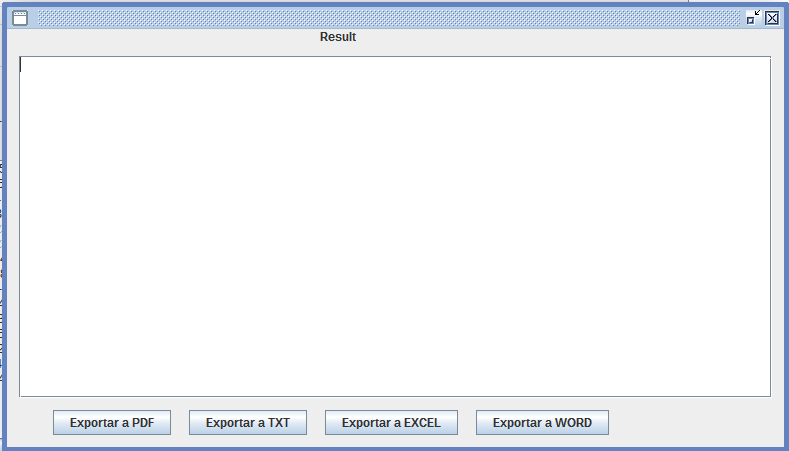
\includegraphics[width=14cm]{fig/resultados}
	\caption{\label{exportar} Interfaz gráfica de ventana de exportación de resultados}
\end{figure}

\begin{figure}[hbtp]
	\centering
	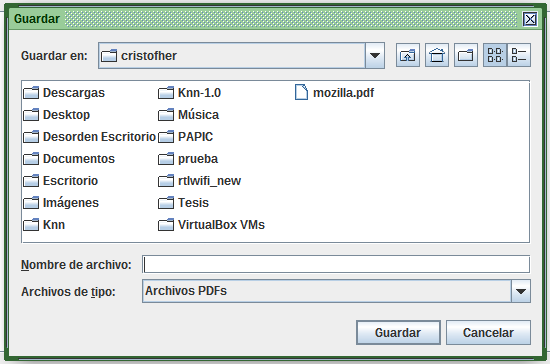
\includegraphics[width=10cm]{fig/guardar}
	\caption{\label{guardar} Interfaz gráfica de ventana de guardar archivo}
\end{figure}


En la figura \ref{guardar} muestra la gráfica de la opción de guardar, cuando se selecciona cualquiera de los tipos de exportación, la gráfica es la misma y es intuitiva de acuerdo al común de las gráficas de exportación de diversos software.
\\
A continuación se muestra extracto de los códigos de exportación de acuerdo a sus formatos, el primer método (Algoritmo \ref{lst:excel}) corresponde al método de exportación de resultados a Excel en formato $.xls$. Para implementar tanto la exportación a Word y a Excel fue necesario incluir una API llamada $POI$ en su \textit{versión 3.16} \cite{poi}, esta API permite que desde una aplicación desarrollada en $Java$ se pueda exportar a diversos formatos como \textit{Word, Hojas de cálculo, Presentaciones, etc} siendo los dos primeros considerados en esta tesis.
\\
El segundo método (Algoritmo \ref{lst:pdf}) es el caso de la exportación a Formato de documento portátil $(PDF)$ fue necesario la importación de $iText$ en su \textit{versión 5} \cite{itex}, esta biblioteca es de código libre (Open Source) desarrollada por iText Group. Esta esta disponible para $Java$ y $C\#$. Esta API termine crear y manipular archivos \textit{PDF - RTF - HTML} en java, siendo el primero considerado para esta tesis. 
\\
El tercer método (Algoritmo \ref{lst:txt}) es el caso de la exportación a archivo de texto plano $(TXT)$, para este tipo de documentos no se utilizo librerías externas debido a que $Java$ posee métodos para la creación y manipulación de estos archivos.   
\\
Los métodos mencionados anteriormente cuentan con una función $obtenerRutaArchivo$, esta permite guardar el archivo con el nombre que le da el usuario y la extensión correspondiente al documento que desea exportar. En caso que el archivo que desea crear ya existe pide la confirmación al usuario si se debe reemplazar el archivo.

\noindent
\begin{algorithm}
\begin{lstlisting}[language=Java] 
public void generarExcel() throws IOException {
    String rutaArchivo = obtenerRutaArchivo("xls", "Archivos Excel");
    if (rutaArchivo != null && jTextArea1.getText().length() != 0) {
        File archivoXLS = new File(rutaArchivo);
        if (archivoXLS.exists()) {
            archivoXLS.delete();
        }
        archivoXLS.createNewFile();
        Workbook libro = new HSSFWorkbook();
        FileOutputStream archivo = new FileOutputStream(archivoXLS);
        Sheet hoja = (Sheet) libro.createSheet("Resultados Knn");
        String texto = jTextArea1.getText();
        String[] lineas = texto.split("\n");
        for (int i = 0; i < lineas.length; i++) {
            Row fila = hoja.createRow(i);
            String[] sublineas = lineas[i].split(" ");
            for (int j = 0; j < sublineas.length; j++) {
                 Cell celda = fila.createCell(j);
                 celda.setCellValue(sublineas[j]);
             }
         }
         libro.write(archivo);
         archivo.close();
         }
}
\end{lstlisting}
\caption{\emph{\label{lst:excel}} Método de exportación de resultados a $Excel$.}
\end{algorithm}



\begin{algorithm}
\begin{lstlisting}[language=Java] 
public void generarPDF() throws IOException, DocumentException {
        String rutaArchivo = obtenerRutaArchivo("pdf", "Archivos PDFs");
        if (rutaArchivo != null) {
            File archivoPDF = new File(rutaArchivo);
            if (archivoPDF.exists()) {
                archivoPDF.delete();
            }
            archivoPDF.createNewFile();
            FileOutputStream archivo = new FileOutputStream(archivoPDF);
            Document documento = new Document();
            PdfWriter.getInstance(documento, archivo);
            documento.open();
            documento.add(new Paragraph("Resultados Knn \n"));
            String texto = jTextArea1.getText();
            String[] lineas = texto.split("\n");
            for (String linea : lineas) {
                documento.add(new Paragraph(linea));
            }
            documento.close();
            JOptionPane.showMessageDialog(null,
                    "El archivo se a guardado Exitosamente",
                    "Informacion", JOptionPane.INFORMATION_MESSAGE);
        }
    }
\end{lstlisting}
\caption{\emph{\label{lst:pdf}} Método de exportación de resultados a $PDF$.}
\end{algorithm}

\begin{algorithm}
\begin{lstlisting}[language=Java] 
    public void generarTXT() throws IOException {
        String rutaArchivo = obtenerRutaArchivo("txt", "Archivo de texto plano TXT");
        try {
            if (rutaArchivo != null) {
                File archivoTXT = new File(rutaArchivo);
                if (archivoTXT.exists()) {
                    archivoTXT.delete();
                }
                try (FileWriter save = new FileWriter(archivoTXT)) {
                    save.write(jTextArea1.getText());
                }
                JOptionPane.showMessageDialog(null,
                        "El archivo se a guardado Exitosamente",
                        "Informacion", JOptionPane.INFORMATION_MESSAGE);
                Desktop.getDesktop().open(archivoTXT);
            }
        } catch (IOException ex) {
            JOptionPane.showMessageDialog(null,
                    "Su archivo no se ha guardado",
                    "Advertencia", JOptionPane.WARNING_MESSAGE);
        }

    }
\end{lstlisting}
\caption{\emph{\label{lst:txt}} Método de exportación de resultados a $TXT$.}
\end{algorithm}

  
\section{Nuevo modulo Añadir menú} 

Para añadir un nuevo método al software además de los que ya cuenta por defecto, el usuario cuenta con un menú de opciones para añadir un método creado por el, pero debe cumplir con ciertos requisitos estipulados de acuerdo a cada uno de los tipos de algoritmo ya sea secuencial o paralelo según la arquitectura.
\\
Cabe mencionar que la realización de este menú, fue realizado a través de una interfaz gráfica en JAVA y su lógica en el lenguaje C, de manera que se dividen las tareas en base al principio divide y vencerás. La interfaz gráfica como se aprecia en la figura \ref{exportar}, donde se aprecia en la parte izquierda de la interfaz los 4 tipos de algoritmos contenidos en el software de modo que si desea ingresar uno nuevo debe indicar a cual de ellos pertenece, de manera similar a la carga de bases de datos y consultas se debe cargar el archivo fuente, este sera visto previamente en el recuadro inferior izquierdo. Además del paso anterior debe especificar el nombre del menú el cual aparecerá en la lista de los menús, para finalizar y lograr añadir correctamente un nuevo método debe presionar el botón \textit{Compile \& add Menu} y el recuadro inferior derecho mostrara información detallada respecto del proceso de compilación, de manera que indica si el proceso fue exitoso o no.  

\begin{figure}[hbtp]
	\centering
	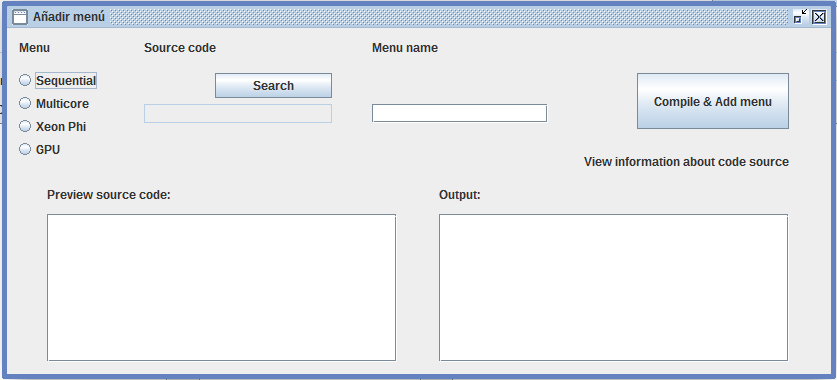
\includegraphics[width=15cm]{fig/add_menu.png}
	\caption{\label{exportar} Interfaz gráfica de ventana Agregar menú}
	\end{figure}

\chapter[Experimentos]{\label{ch:experimentos}Experimentos}

texto...

\chapter[Conclusiones]{\label{ch:conclusiones}Conclusiones}

texto...


\section{Trabajos Futuros}

\begin{itemize}
\item uno...
\item dos...
\item N...
\end{itemize}


\section{Contribuciones de la Tesis}

\begin{itemize}
\item uno...
\item dos...
\item N...
\end{itemize}




%%% Apendices Opcionales  %%%%
%\appendixpage
%\begin{appendices}
%\input{anexo-1}
%\input{anexo-2}
%\end{appendices}




\backmatter

\bibliographystyle{alpha}
\bibliography{biblio}

\end{document}


